\chapter{Studii de Caz de Explicabilitate}
\label{ch:explainability}

Acest capitol testează afirmații specifice din Capitolul~\ref{ch:results} prin diagnostice țintite, în loc să se bazeze doar pe metricile agregate.

\section{Localizarea Erorii de Reconstrucție pe Yahoo A3}
\label{sec:explain-yahoo}

Discuția despre A3 din Capitolul~\ref{ch:results} atribuie avantajul Transformer Bottleneck Autoencoder-ului față de LSTM Autoencoder (AP 0.663 vs.\ 0.392, ROC-AUC 0.813 vs.\ 0.566) unei diferențe dintre cele două bottleneck-uri: LSTM Autoencoder comprimă o fereastră întreagă de 64 de pași într-o singură stare ascunsă finală, ceea ce ar trebui să distrugă informația de fază sezonieră, în timp ce auto-atenția globală a Transformer-ului ar trebui să păstreze suficientă informație pozițională pentru a localiza eroarea precis, la pasul unde faza este încălcată. Se presupune deci că, pentru ferestrele A3 anormale, LSTM Autoencoder produce o eroare difuzată uniform pe toți pașii, în timp ce eroarea Transformer-ului prezintă un vârf ascuțit, localizat, la poziția unde tiparul sezonier e încălcat.

O verificare calitativă preliminară (hărți termice ale erorii per pas temporal -- Anexa~\ref{ch:yahoo-heatmap-appendix}) e în linii mari consistentă cu ipoteza, dar insuficientă pentru a o confirma: fiecare panou e normalizat pe propria scală de culoare, iar valorile de eroare ale LSTM Autoencoder-ului sunt, ca magnitudine, aproximativ duble față de cele ale Transformer-ului pe tot parcursul. E necesară o măsură cantitativă, invariantă la scala absolută.

\subsection{Verificare Cantitativă: Coeficientul Gini al Concentrării Erorii}

Pentru a separa concentrarea reală a erorii de un artefact al diferenței de magnitudine globală, cele 64 de erori pătratice per pas temporal ale fiecărei ferestre anormale au fost sumarizate printr-un coeficient Gini -- o măsură standard de inegalitate (folosită inițial pentru distribuții de venit), invariantă la scala absolută a datelor. Pentru cele 64 de valori de eroare ale unei ferestre, sortate crescător, un Gini de 0 înseamnă eroare răspândită perfect uniform pe fiecare pas temporal, iar un Gini de 1 înseamnă concentrare totală la un singur pas.

Pentru $n$ erori pătratice per pas temporal $x_1 \le x_2 \le \dots \le x_n$ sortate crescător (aici $n=64$), coeficientul Gini se calculează ca

\begin{equation}
G = \frac{2 \sum_{i=1}^{n} i \, x_i}{n \sum_{i=1}^{n} x_i} - \frac{n+1}{n}.
\label{eq:gini}
\end{equation}

Calculat pe întreaga populație de 14{,}449 ferestre A3 anormale, cele două modele se separă clar:

\begin{center}
\begin{tabular}{@{}lll@{}}
\toprule
 & Gini Mediu & Gini Median \\
\midrule
LSTM Autoencoder & 0.566 & 0.606 \\
Transformer Bottleneck Autoencoder & 0.721 & 0.724 \\
\bottomrule
\end{tabular}
\end{center}

\begin{figure}[H]
\centering
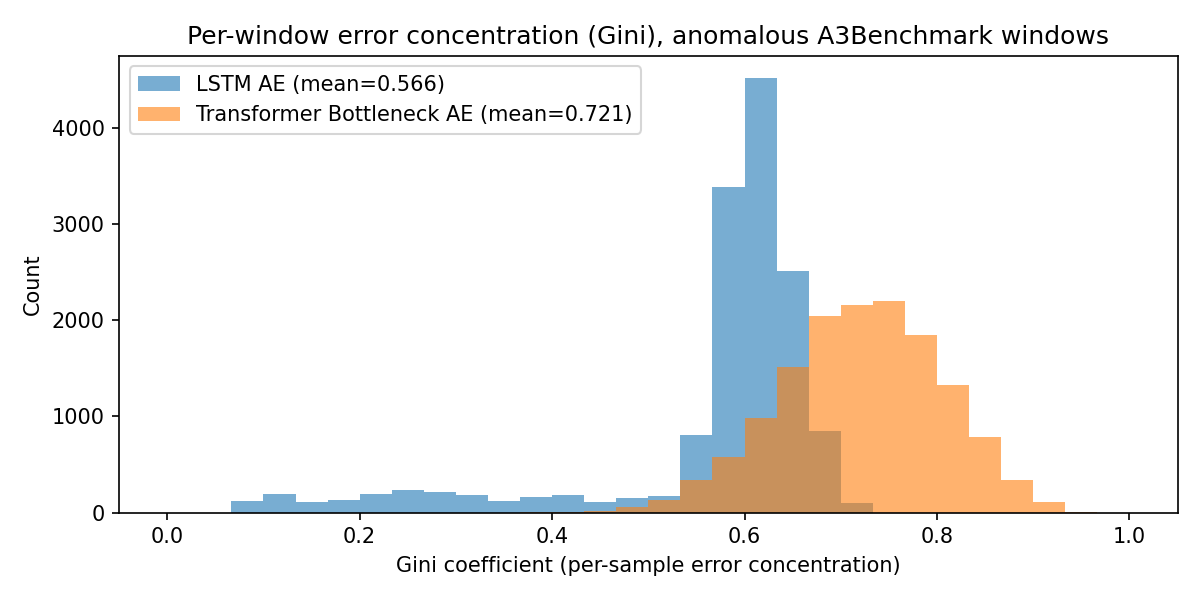
\includegraphics[width=0.46\textwidth]{../../data/explainability/yahoo_A3Benchmark_lstm_vs_transformer/5/gini_comparison.png}
\caption{Distribuția coeficienților Gini per fereastră, pe toate cele 14{,}449 ferestre A3 anormale. Distribuția Transformer-ului este unimodală și deplasată spre concentrare ridicată (Gini $>0.6$); distribuția LSTM Autoencoder-ului este bimodală, cu o majoritate grupată aproape de intervalul Transformer-ului, dar cu o populație secundară distinctă răspândită la valori Gini scăzute.}
\label{fig:explain-gini}
\end{figure}

Aceasta confirmă ipoteza inițială în mare: eroarea Transformer-ului e mai concentrată decât cea a LSTM Autoencoder-ului pe întreaga populație anormală, nu doar în puținele exemple arătate întâmplător de o hartă termică.
Dar distribuția din Figura~\ref{fig:explain-gini} relevă un detaliu interesant -- valorile Gini ale LSTM Autoencoder-ului sunt \emph{bimodale}, nu deplasate uniform în jos. O majoritate a ferestrelor sale se grupează practic în același interval de concentrare ridicată ca al Transformer-ului (Gini $\approx 0.6$, capacitate de localizare comparabilă), în timp ce o populație secundară distinctă se situează la Gini scăzut ($<0.4$), unde eroarea e cu adevărat difuzată aproape uniform pe toată fereastra. Aceasta indică faptul că mecanismul de distrugere a fazei nu e o proprietate uniformă a fiecărei reconstrucții LSTM Autoencoder, ci un fenomen care afectează un subset specific de ferestre -- și această subpopulație, nu o degradare generală, e responsabilă pentru scăderea AP-ului și ROC-AUC-ului agregat al LSTM Autoencoder-ului sub cel al Transformer-ului, întrucât pe restul majoritar al ferestrelor cele două modele localizează eroarea la fel de bine.




\section{Regimuri de Caracteristici Disjuncte: AE+Context vs.\ Temporal IForest}
\label{sec:explain-disjoint-regime}

Discuția despre CIC-IDS2017 din Capitolul~\ref{ch:results} propune combinarea AE+Context (puternic pe DDoS și PortScan) cu Temporal IForest (puternic pe clasele DoS lente și, cu rezerve, pe Heartbleed) într-un ansamblu, întrucât cele două ar trebui să opereze pe mulțimi de caracteristici disjuncte -- caracteristici de context al gazdei versus o fereastră temporală de 16 fluxuri.

\paragraph{O scurtă introducere la SHAP.} SHAP (\emph{SHapley Additive exPlanations}) atribuie fiecărui eșantion câte o valoare per caracteristică de intrare, reprezentând cât de mult a influențat acea caracteristică ieșirea modelului. Semnul arată direcția împingerii (spre normal sau spre anormal, în funcție de convenția ieșirii explicate -- precizată separat pentru fiecare model mai jos, întrucât cele două nu coincid), iar magnitudinea arată contribuția relativă la celelalte caracteristici ale aceluiași eșantion.

O \emph{diagramă beeswarm} (Figurile~\ref{fig:explain-temporal-beeswarm} și~\ref{fig:explain-ae-context-portscan-shap}) arată atribuirea SHAP pe un eșantion de puncte de test, câte un rând per caracteristică, ordonate descrescător după importanță; pe fiecare rând, fiecare punct e un eșantion, poziționat orizontal după propria valoare SHAP și colorat după propria valoare a caracteristicii (albastru pentru valoare mică, roșu pentru valoare mare). Pentru definiția matematică și originea din teoria jocurilor cooperative: \parencite{lundberg2017unified}; pentru o descriere mai accesibilă și detalii despre construcția diagramelor: documentația SHAP~\cite{shap_docs}.

Se presupune deci că (1) dacă Temporal IForest exploatează cu adevărat structura dintre pașii temporali, scorul său per fereastră ar trebui să poarte informație despre eticheta \emph{ultimului} flux -- cel combinat cu scorul lui AE+Context -- nu doar despre dacă \emph{vreun} flux din fereastra de 16 e un atac, deci atribuirea sa SHAP nu ar trebui să se prăbușească pe acel flux final; și (2) avantajul lui AE+Context pe propriile sale clase puternice provine din cele 9 caracteristici de context al gazdei, care ar trebui deci să apară printre caracteristicile cu cea mai mare medie $|\text{SHAP}|$.

O validare suplimentară -- verificarea faptului că scorul lui Temporal IForest rămâne informativ și sub o etichetare mai strictă, per ultimul flux, nu doar sub eticheta permisivă "oricare-din-16" -- este detaliată în Anexa~\ref{ch:temporal-iforest-last-flow-validation}.



\subsection{Temporal IForest: Atribuire SHAP pe Toată Fereastra}
\label{sec:explain-temporal-window}

Temporal IForest e antrenat pe ferestre aplatizate de 16 fluxuri, deci valorile SHAP ale lui \texttt{TreeExplainer}~\parencite{lundberg2020local} pe intrarea aplatizată se descompun curat înapoi într-un cub (fereastră, pas temporal, caracteristică). Pentru fiecare din cele patru clase, SHAP a fost calculat pe 200 de ferestre; magnitudinea atribuirii a fost sumată pe caracteristici per pas temporal, iar caracteristicile cu cea mai mare contribuție au fost reprezentate pe toți cei 16 pași pentru a verifica dacă poartă o atribuire cu semn consistent pe toată fereastra, nu doar aproape de final.

\begin{figure}[H]
\centering
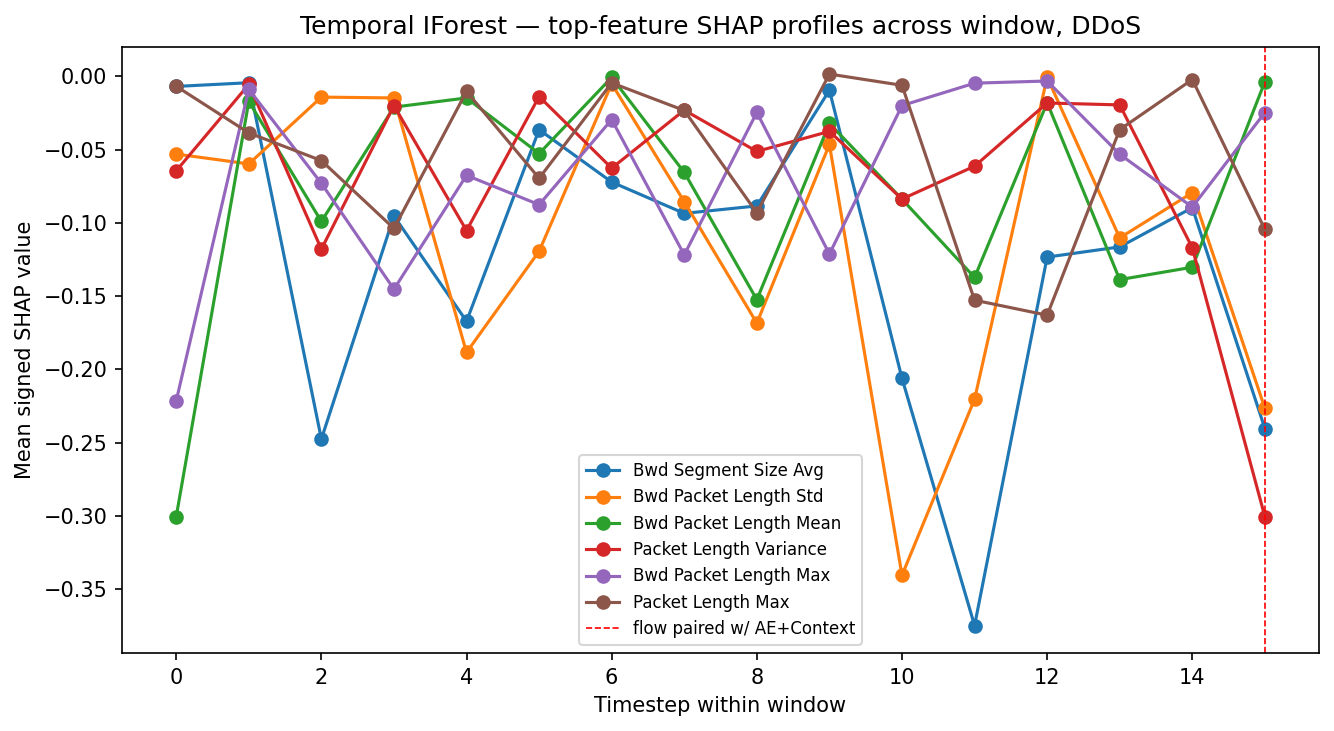
\includegraphics[width=0.38\textwidth,keepaspectratio]{../../data/explainability/cicids_temporal_shap/1/ddos_top_feature_profiles.png}%
\hspace{0.02\textwidth}%
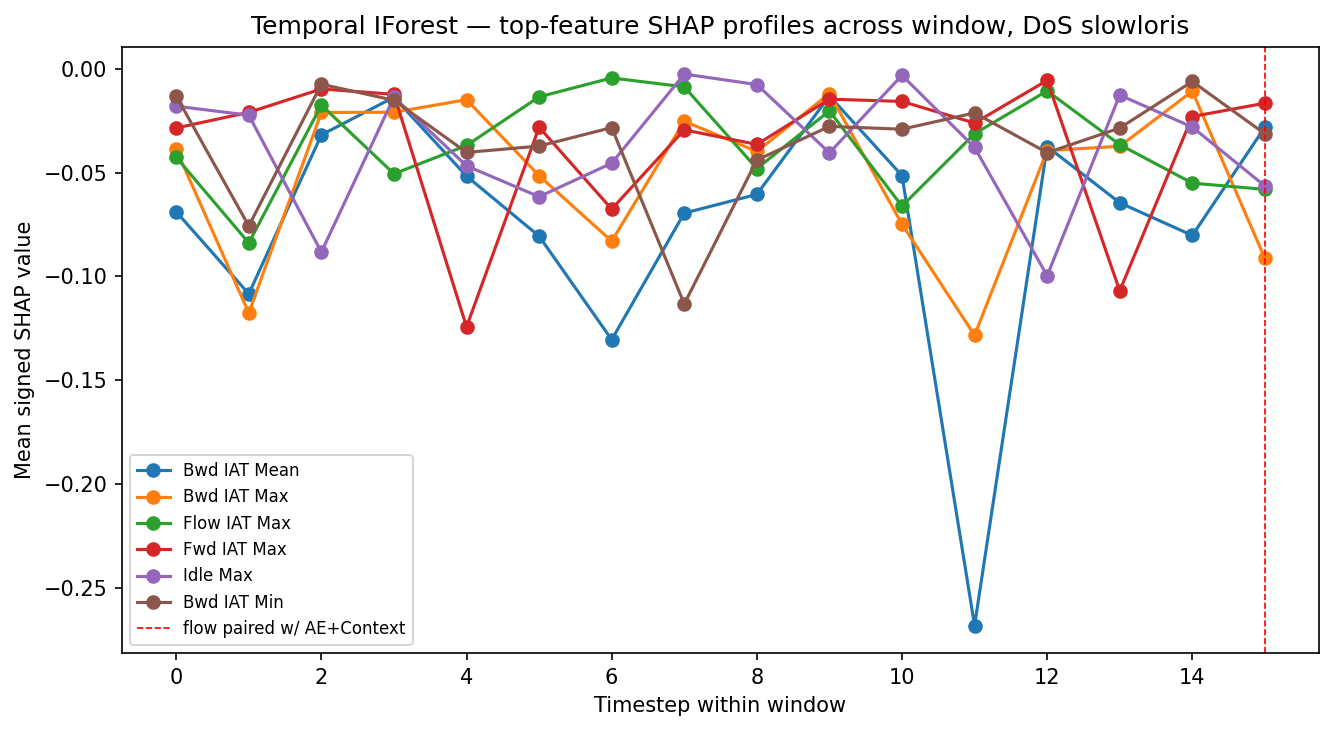
\includegraphics[width=0.38\textwidth,keepaspectratio]{../../data/explainability/cicids_temporal_shap/1/dos_slowloris_top_feature_profiles.png}

\caption{Temporal IForest -- valoarea medie SHAP per pas temporal pentru cele șase caracteristici cu cea mai mare atribuire, ferestre DDoS (stânga) și ferestre DoS slowloris (dreapta). În ambele cazuri atribuirea este negativă (anormală), recurentă cu semn consistent pe majoritatea celor 16 pași temporali, și nu se concentrează pe fluxul final (linia roșie punctată) -- fluxul combinat cu scorul lui AE+Context în ansamblul propus.}
\label{fig:explain-temporal-shap}
\end{figure}

Doi diagnostici suplimentari (Anexa~\ref{ch:temporal-shap-extra}) confirmă că ultimul pas temporal nu domină atribuirea (6--8\% din masa totală, aproape de referința uniformă de 6.25\% pentru o fereastră de 16 pași).
Caracteristicile principale se potrivesc cu mecanismul cunoscut al fiecărui atac: atribuirea DDoS/GoldenEye se concentrează pe lungimea pachetelor pe direcția inversă (\texttt{Bwd Packet Length Std/Mean/Max}), consistent cu un flux volumetric; atribuirea Slowhttptest/slowloris se concentrează pe timpul între sosiri (\texttt{Fwd/Bwd IAT Std/Max}), consistent cu comportamentul lent, de menținere a conexiunii -- confirmând ipoteza.



\subsection{AE+Context: SHAP Dominat de Caracteristici de Context al Gazdei}

SHAP a fost calculat cu \texttt{GradientExplainer} pe eroarea de reconstrucție a lui AE+Context, pe câte 200 de eșantioane din PortScan și DDoS, iar cele 15 caracteristici cu cea mai mare medie $|\text{SHAP}|$ au fost clasate per clasă.

\begin{figure}[H]
\centering
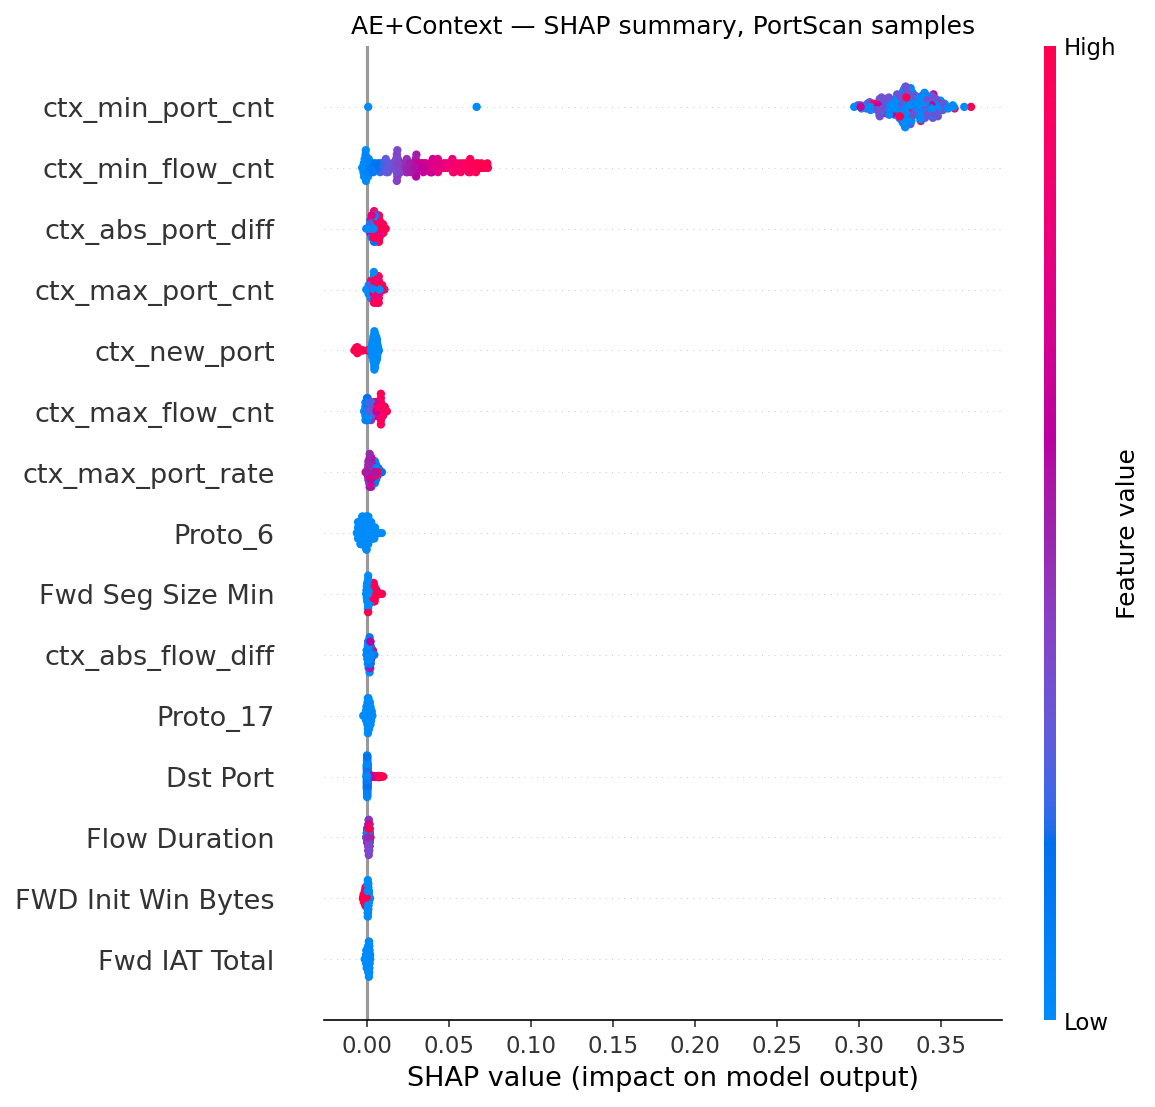
\includegraphics[width=0.44\textwidth]{../../data/explainability/cicids_shap_portscan/5/autoencoder_context_portscan_shap.png}
\caption{AE+Context -- diagramă sumară SHAP, eșantioane PortScan. \texttt{ctx\_min\_port\_cnt} domină printr-un cluster strâns, uniform pozitiv, bine separat de orice altă caracteristică; rândurile de top rămase sunt aproape în întregime caracteristici de context al gazdei.}
\label{fig:explain-ae-context-portscan-shap}
\end{figure}

\begin{center}
\begin{tabular}{@{}lcc@{}}
\toprule
 & Caracteristici de context în top 15 & Caracteristica principală (medie $|\text{SHAP}|$) \\
\midrule
PortScan & 8/15 & \texttt{ctx\_min\_port\_cnt} (0.324) \\
DDoS     & 7/15 & \texttt{ctx\_min\_port\_cnt} (0.234) \\
\bottomrule
\end{tabular}
\end{center}

Pentru ambele clase, \texttt{ctx\_min\_port\_cnt} și \texttt{ctx\_min\_flow\_cnt} domină cu aproximativ un ordin de mărime peste orice caracteristică de flux obișnuită. Șase din cele nouă caracteristici de context apar în listele de top 15 ale ambelor clase, doar \texttt{ctx\_min\_port\_rate} lipsind din amândouă -- confirmând premisa: avantajul lui AE+Context pe aceste clase e determinat aproape în întregime de dovezi de context al gazdei indisponibile lui Temporal IForest.



\subsection{Construirea Scorului Combinat}
\label{sec:explain-ensemble-build}

Realizarea ansamblului schițat în Capitolul~\ref{ch:results} necesită combinarea, pentru fiecare flux $f$, a scorului propriu al lui AE+Context cu scorul lui Temporal IForest pentru fereastra de 16 fluxuri care se \emph{încheie} la $f$. Cele două scoruri brute nu pot fi combinate direct (eroare de reconstrucție fără scală fixă vs.\ lungime medie de cale negată), deci e necesară o normalizare -- calculată doar pe scorurile de antrenare \emph{benigne} ale fiecărui model, niciodată pe date de test, pentru a evita scurgerea informației de anomalie în combinare.

Au fost testate două reguli: \textbf{votarea ponderată (soft voting)}, $s_{\text{soft}}(f) = w \cdot \hat{s}_{AE}(f) + (1-w) \cdot \hat{s}_{IF}(f)$, variind $w \in \{0.3, \dots, 0.7\}$; și \textbf{regula maximului}, $s_{\text{max}}(f) = \max(\hat{s}_{AE}(f), \hat{s}_{IF}(f))$ -- un combinator de tip OR, reflectând ideea că încrederea oricărui model, singură, ar trebui să fie suficientă.

Cele două scoruri au fost normalizate pe rang -- mapând fiecare scor de test la percentila sa în distribuția scorurilor proprii de antrenare benignă -- în locul standardizării $z$, care s-a dovedit o fundătură (normalizarea pe rang mărginește fiecare scor la $[0,1]$, indiferent de valoarea brută). Detalii: Anexa~\ref{ch:ensemble-score-alignment}.

\subsection{Acoperire per Clasă vs.\ AP Agregat}
\label{sec:explain-ensemble-results}

\begin{center}
\begin{tabular}{@{}lccccc@{}}
\toprule
 & DDoS & PortScan & GoldenEye & Slowhttptest & slowloris \\
\midrule
AE+Context singur         & 0.882 & \textbf{0.924} & 0.292 & 0.013 & 0.025 \\
Temporal IForest singur   & \textbf{0.956} & 0.123 & 0.611 & 0.578 & 0.560 \\
Regula maximului (rang)   & 0.882 & 0.923 & 0.292 & 0.060 & 0.083 \\
Votare ponderată $w=0.4$ (rang) & 0.977 & 0.228 & \textbf{0.801} & \textbf{0.205} & \textbf{0.319} \\
Votare ponderată $w=0.7$ (rang) & 0.977 & 0.358 & 0.821 & 0.140 & 0.245 \\
\bottomrule
\end{tabular}
\end{center}

AP-ul agregat \emph{favorizează} de fapt variantele care se schimbă cel mai puțin: regula maximului (0.943) și AE+Context singur (0.941) depășesc votarea ponderată $w=0.4$ (0.841), pur și simplu pentru că DDoS și PortScan totalizează peste 250{,}000 din cele $\sim$434{,}000 de fluxuri pozitive, față de doar 13{,}000 pentru GoldenEye, Slowhttptest și slowloris împreună.

Nicio regulă nu e un câștig gratuit, dar votarea ponderată pare alegerea mai pertinentă pentru un ansamblu motivat de acoperire: clasa sa cea mai \emph{slabă} (0.205, Slowhttptest, la $w=0.4$) depășește propriile clase cele mai slabe ale ambelor modele singure -- 0.013 (AE+Context) și 0.123 (Temporal IForest) -- ceva ce niciun model singur sau regula maximului nu realizează. E o realizare autentică, deși parțială, a ideii de ansamblu din Capitolul~\ref{ch:results}: votarea ponderată pe rang lărgește pragul minim de acoperire, cu costul detecției PortScan.
